\documentclass{beamer}

% for themes, etc.
\mode<presentation>
{ \usetheme{metropolis} }
%{ \usetheme{Torino} }
%{ \usetheme{boxes} }

\usepackage{times}  % fonts are up to you
\usepackage{graphicx}
\usepackage{color,colortbl}

\definecolor{MRed}{rgb}{1,.6,.6}
% these will be used later in the title page
\title{ALICE MUON Software for run 3}
\author{Sean Murray \\
    Physics \\
    University of Cape Town 
}
\date{July 6, 2016}

% note: do NOT include a \maketitle line; also note that this title
% material goes BEFORE the \begin{document}

% have this if you'd like a recurring outline
\AtBeginSection[]  % "Beamer, do the following at the start of every section"
{
\begin{frame}<beamer> 
\frametitle{Outline} % make a frame titled "Outline"
\tableofcontents[currentsection]  % show TOC and highlight current section
\end{frame}
}

\begin{document}

% this prints title, author etc. info from above
\begin{frame}
\titlepage
\end{frame}

\section{ALICE}

\begin{frame}
\frametitle{ALICE}

  \center{
  
\includegraphics[scale=0.35,trim={5cm 2cm 3cm 4cm},clip]{images/pg_0004.pdf}
  }
\end{frame}


\section{O2 and Run3}
\begin{frame}
\frametitle{O2 Online/Offline}
We will not go into depth, this is a whole other presentation.
Important numbers to take away :
\begin{itemize}
  \item 50kHz event rate.
  \item 1.1 TB/s agregate data rate, spikes upto 15.
  \item continuous read out for most detectors, tpc and muon sharing electronics.
  \item Completely new framework.
  \item merge HLT, data acquisition and offline into 1 code base and platform.
  \item calibration and reconstruction online.
  \item Collaboration with FAIR for new framework.
\end{itemize}

\end{frame}
\begin{frame}
  \frametitle{O2 Farm}
  \center{
  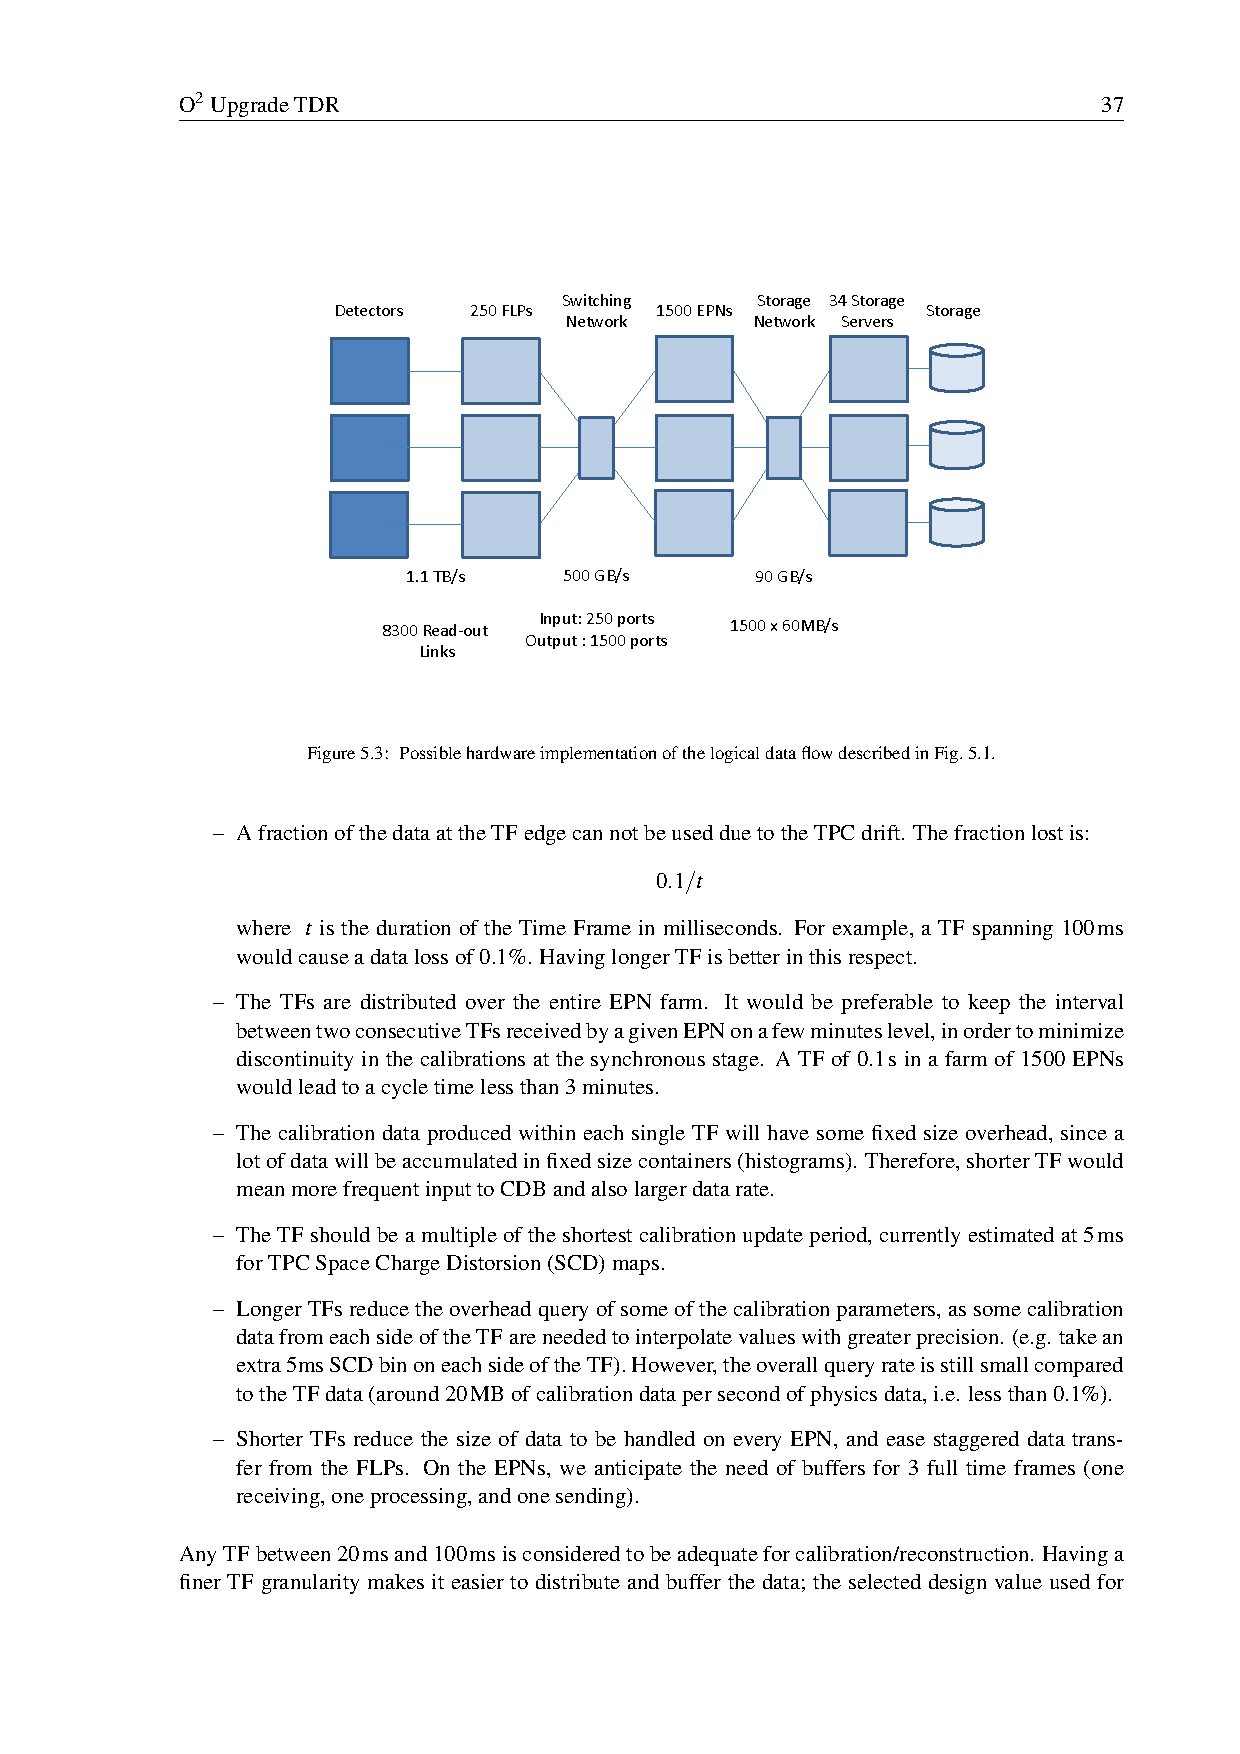
\includegraphics[scale=0.7,trim={3cm 18cm 3cm 3cm},clip]{images/ALICE_TDR-019_49.pdf}
  }
\end{frame}

\begin{frame}
  \frametitle{MUON Links}
  \tiny{\begin{tabular}{|l|l|r|r|r|l|r|r|}
   Detector  &      Link    &  \multicolumn{3}{c}{ Number of links}   &     Read-out &   \multicolumn{2}{c}{Number of boards} \\
             &      type    & DDL1& DDL2 &  GBT  &  board type&   C-RORC& CRU \\ \hline\hline
    ACO      &     DDL1     &  1  &      &       &  C-RORC    &      1   &   \\ 
    CPV      &     DDL1     &  6  &      &       &  C-RORC    &      1   &\\ 
    CTP      &    GBT       &     &      &    14 &  CRU       &          &     1\\ 
    EMC      &   DDL2       &     &   20 &       &  C-RORC    &      4   &\\ 
    FIT      &     DDL2     &     &    2 &       &  C-RORC    &      1   &\\ 
    HMP      &     DDL1     &  14 &      &       &  C-RORC    &      4   &\\ 
    ITS      &     GBT      &     &      &   495 &  CRU       &          &               23\\ 
\rowcolor{MRed}    MCH      &     GBT      &     &      &   550 &  CRU       &          &               25\\ 
\rowcolor{MRed}    MFT      &     GBT      &     &      &   304 &  CRU       &          &               14\\ 
\rowcolor{MRed}    MID      &     GBT      &     &      &    32 &  CRU       &          &                2\\ 
    PHS      &     DDL2     &     &      &    16 &  C-RORC    &     4    &\\ 
    TOF      &     GBT      &     &      &    72 &  CRU       &          &               3\\ 
    TPC      &     GBT      &     &      &  5832 &  CRU       &          &             324\\ 
    TRD      &     Custom   &     &      &  1044 &  CRU       &          &              54\\ 
    ZDC      &     GBT      &     &      &     1 &  CRU       &          &               1\\  \hline
    Total    &               & 21 &  38  &  8344 &            &   15     &          447\\ 
            \end{tabular}}\\
            Muon therefore gets 5 FLP's
\end{frame}

\begin{frame}
\frametitle{ALICE MUON Arm}
  \center{
  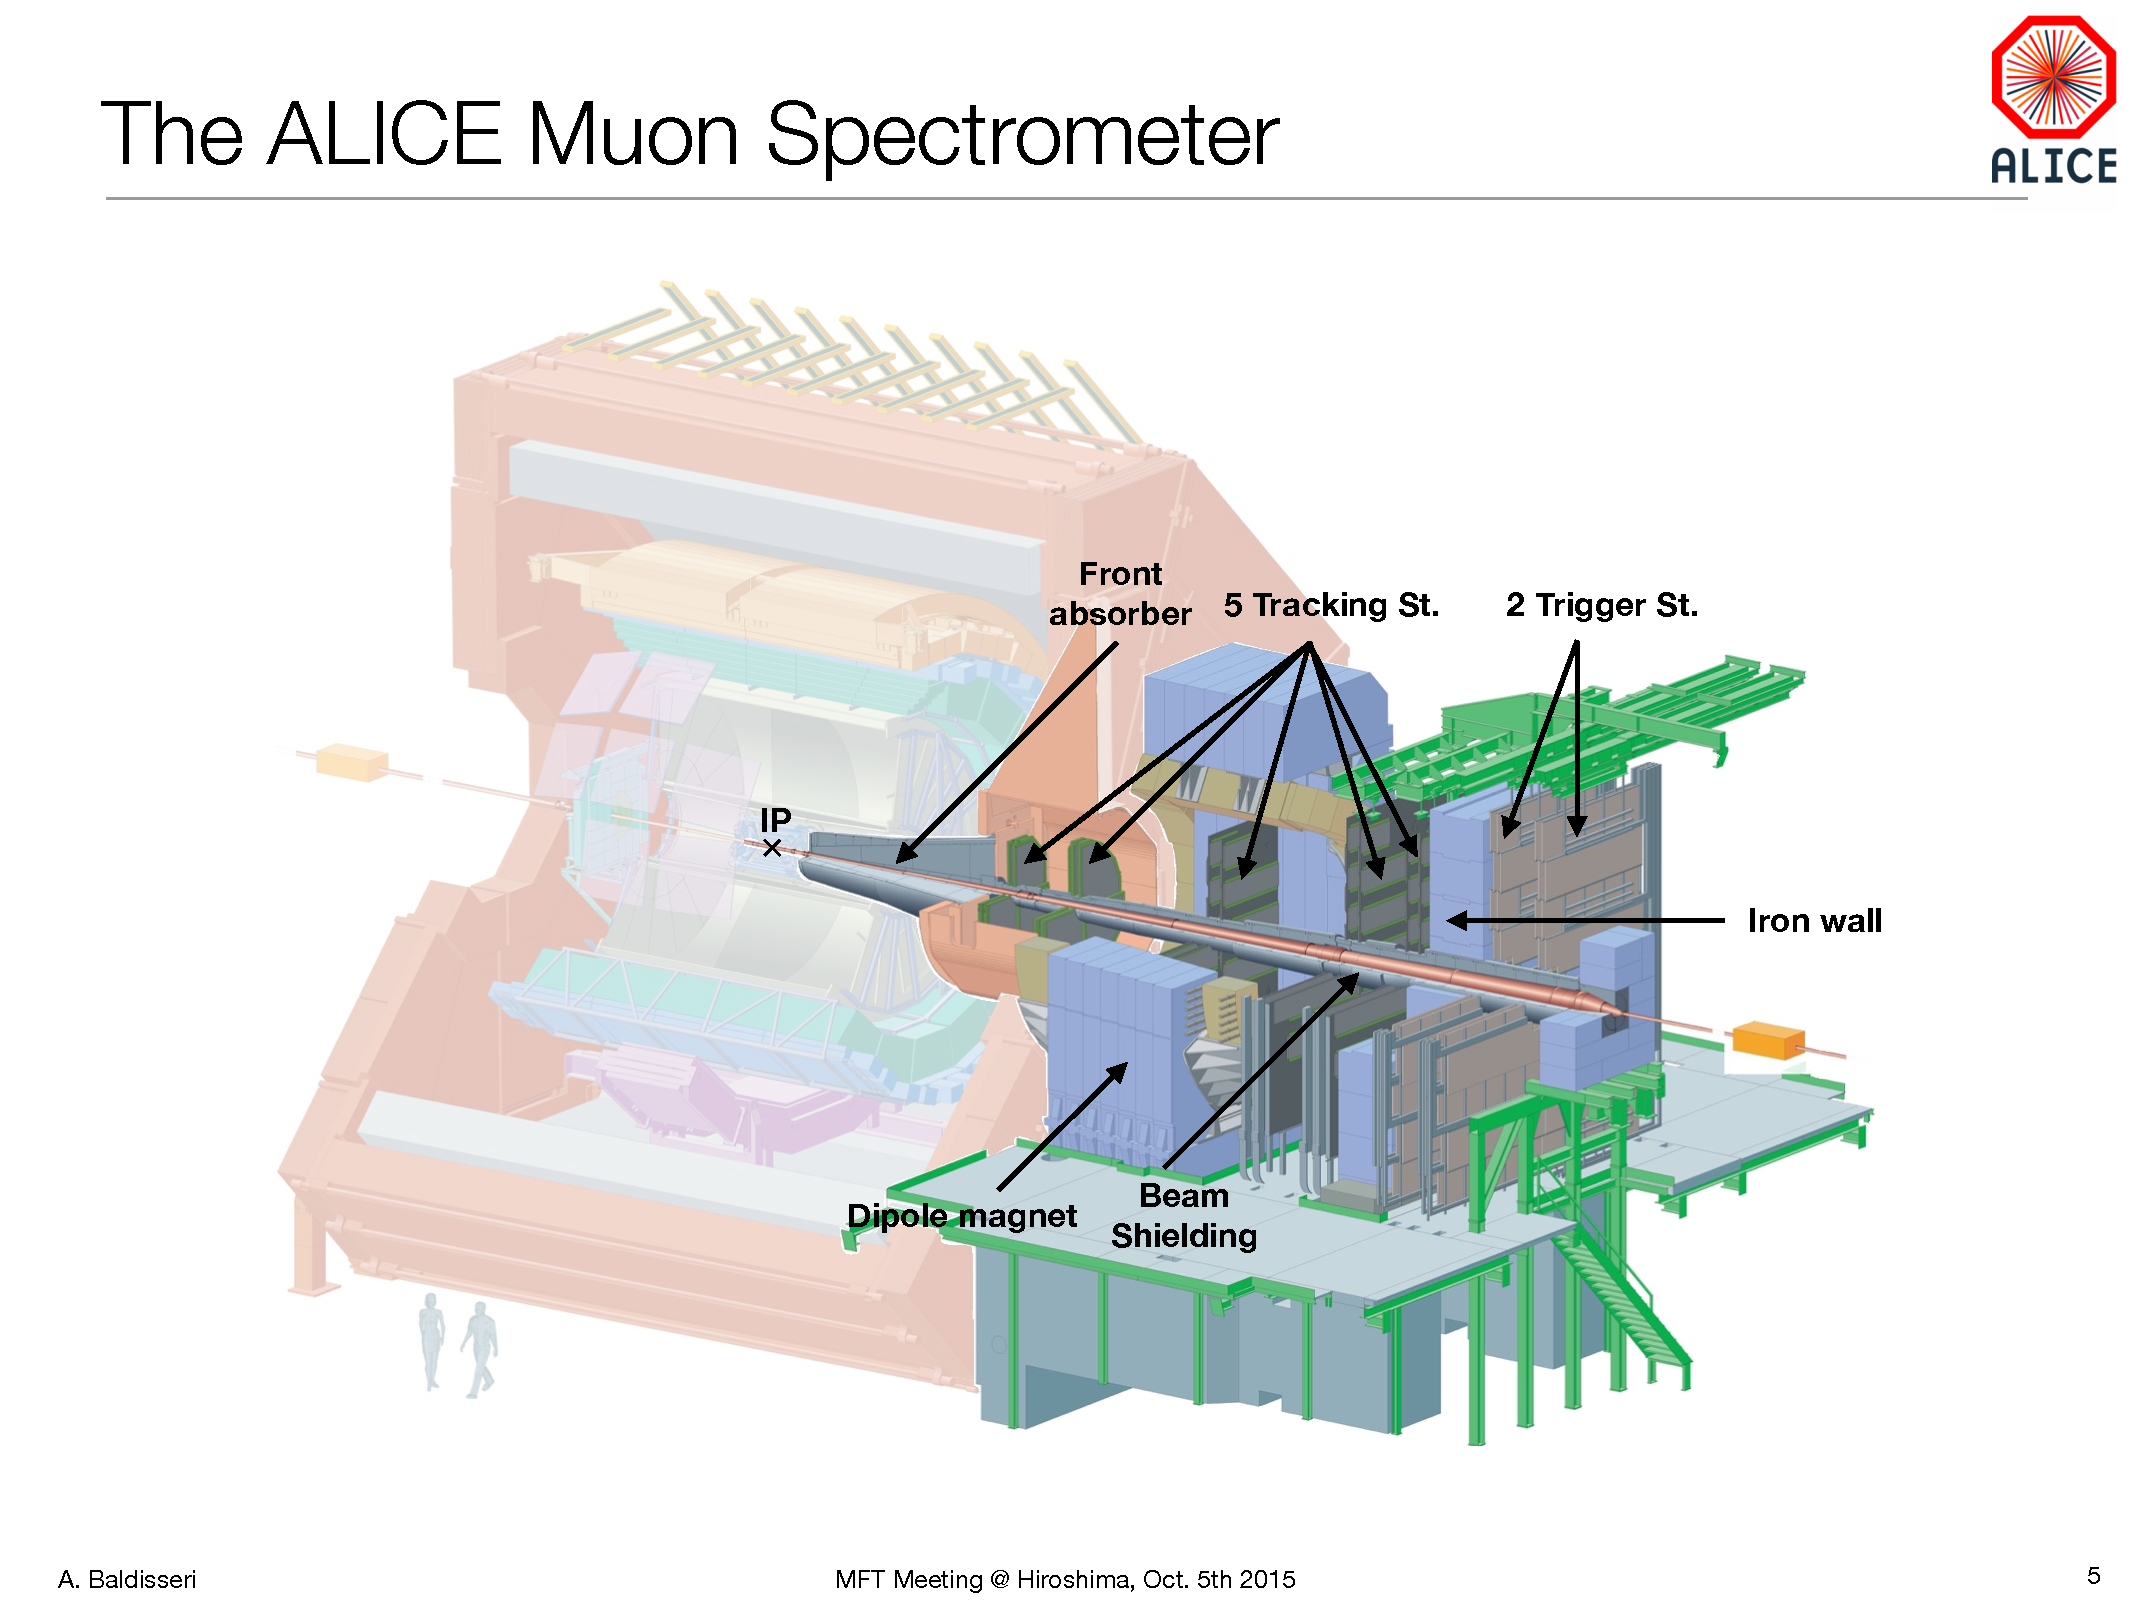
\includegraphics[scale=0.35,trim={3cm 1cm 3cm 4cm},clip]{images/pg_0005.pdf}
  }
\end{frame}

\section{ALICE Muons}

\begin{frame}
  \frametitle{ALICE MUON diagram}

  \center{
  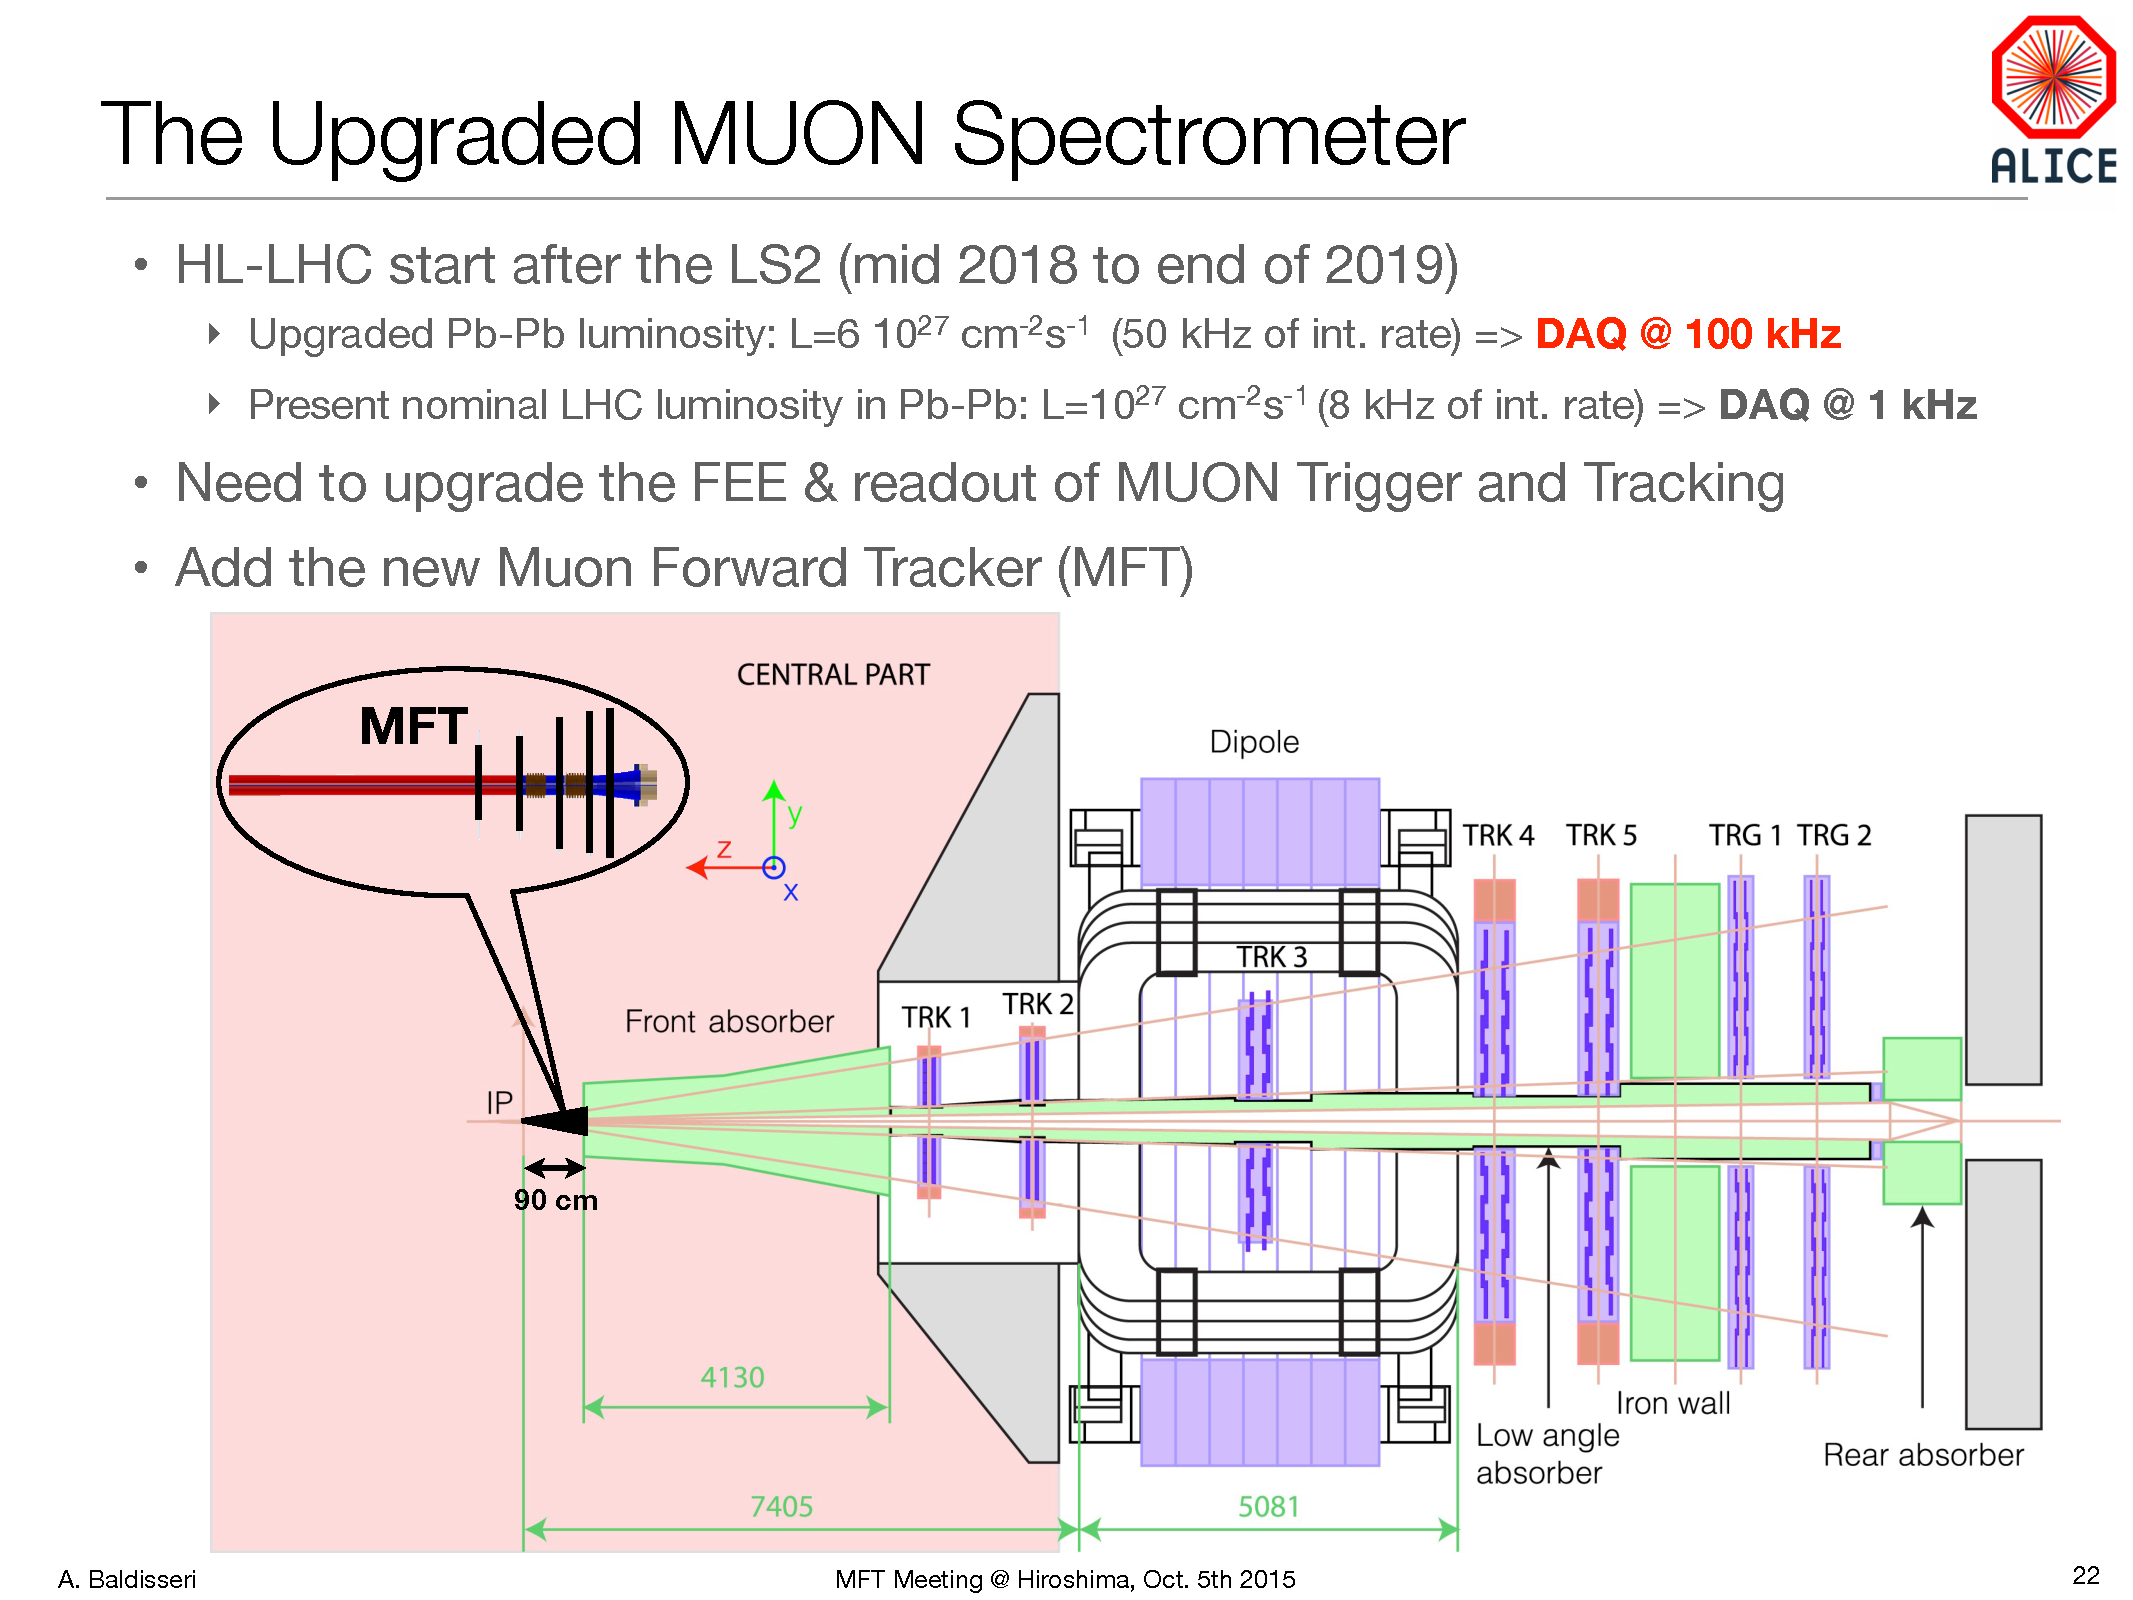
\includegraphics[scale=0.35,trim={2cm 0.75cm 1cm 10cm},clip]{images/pg_0022.pdf}
  }

\end{frame}

\begin{frame}
\frametitle{Detector Structure Station1}
\centering{
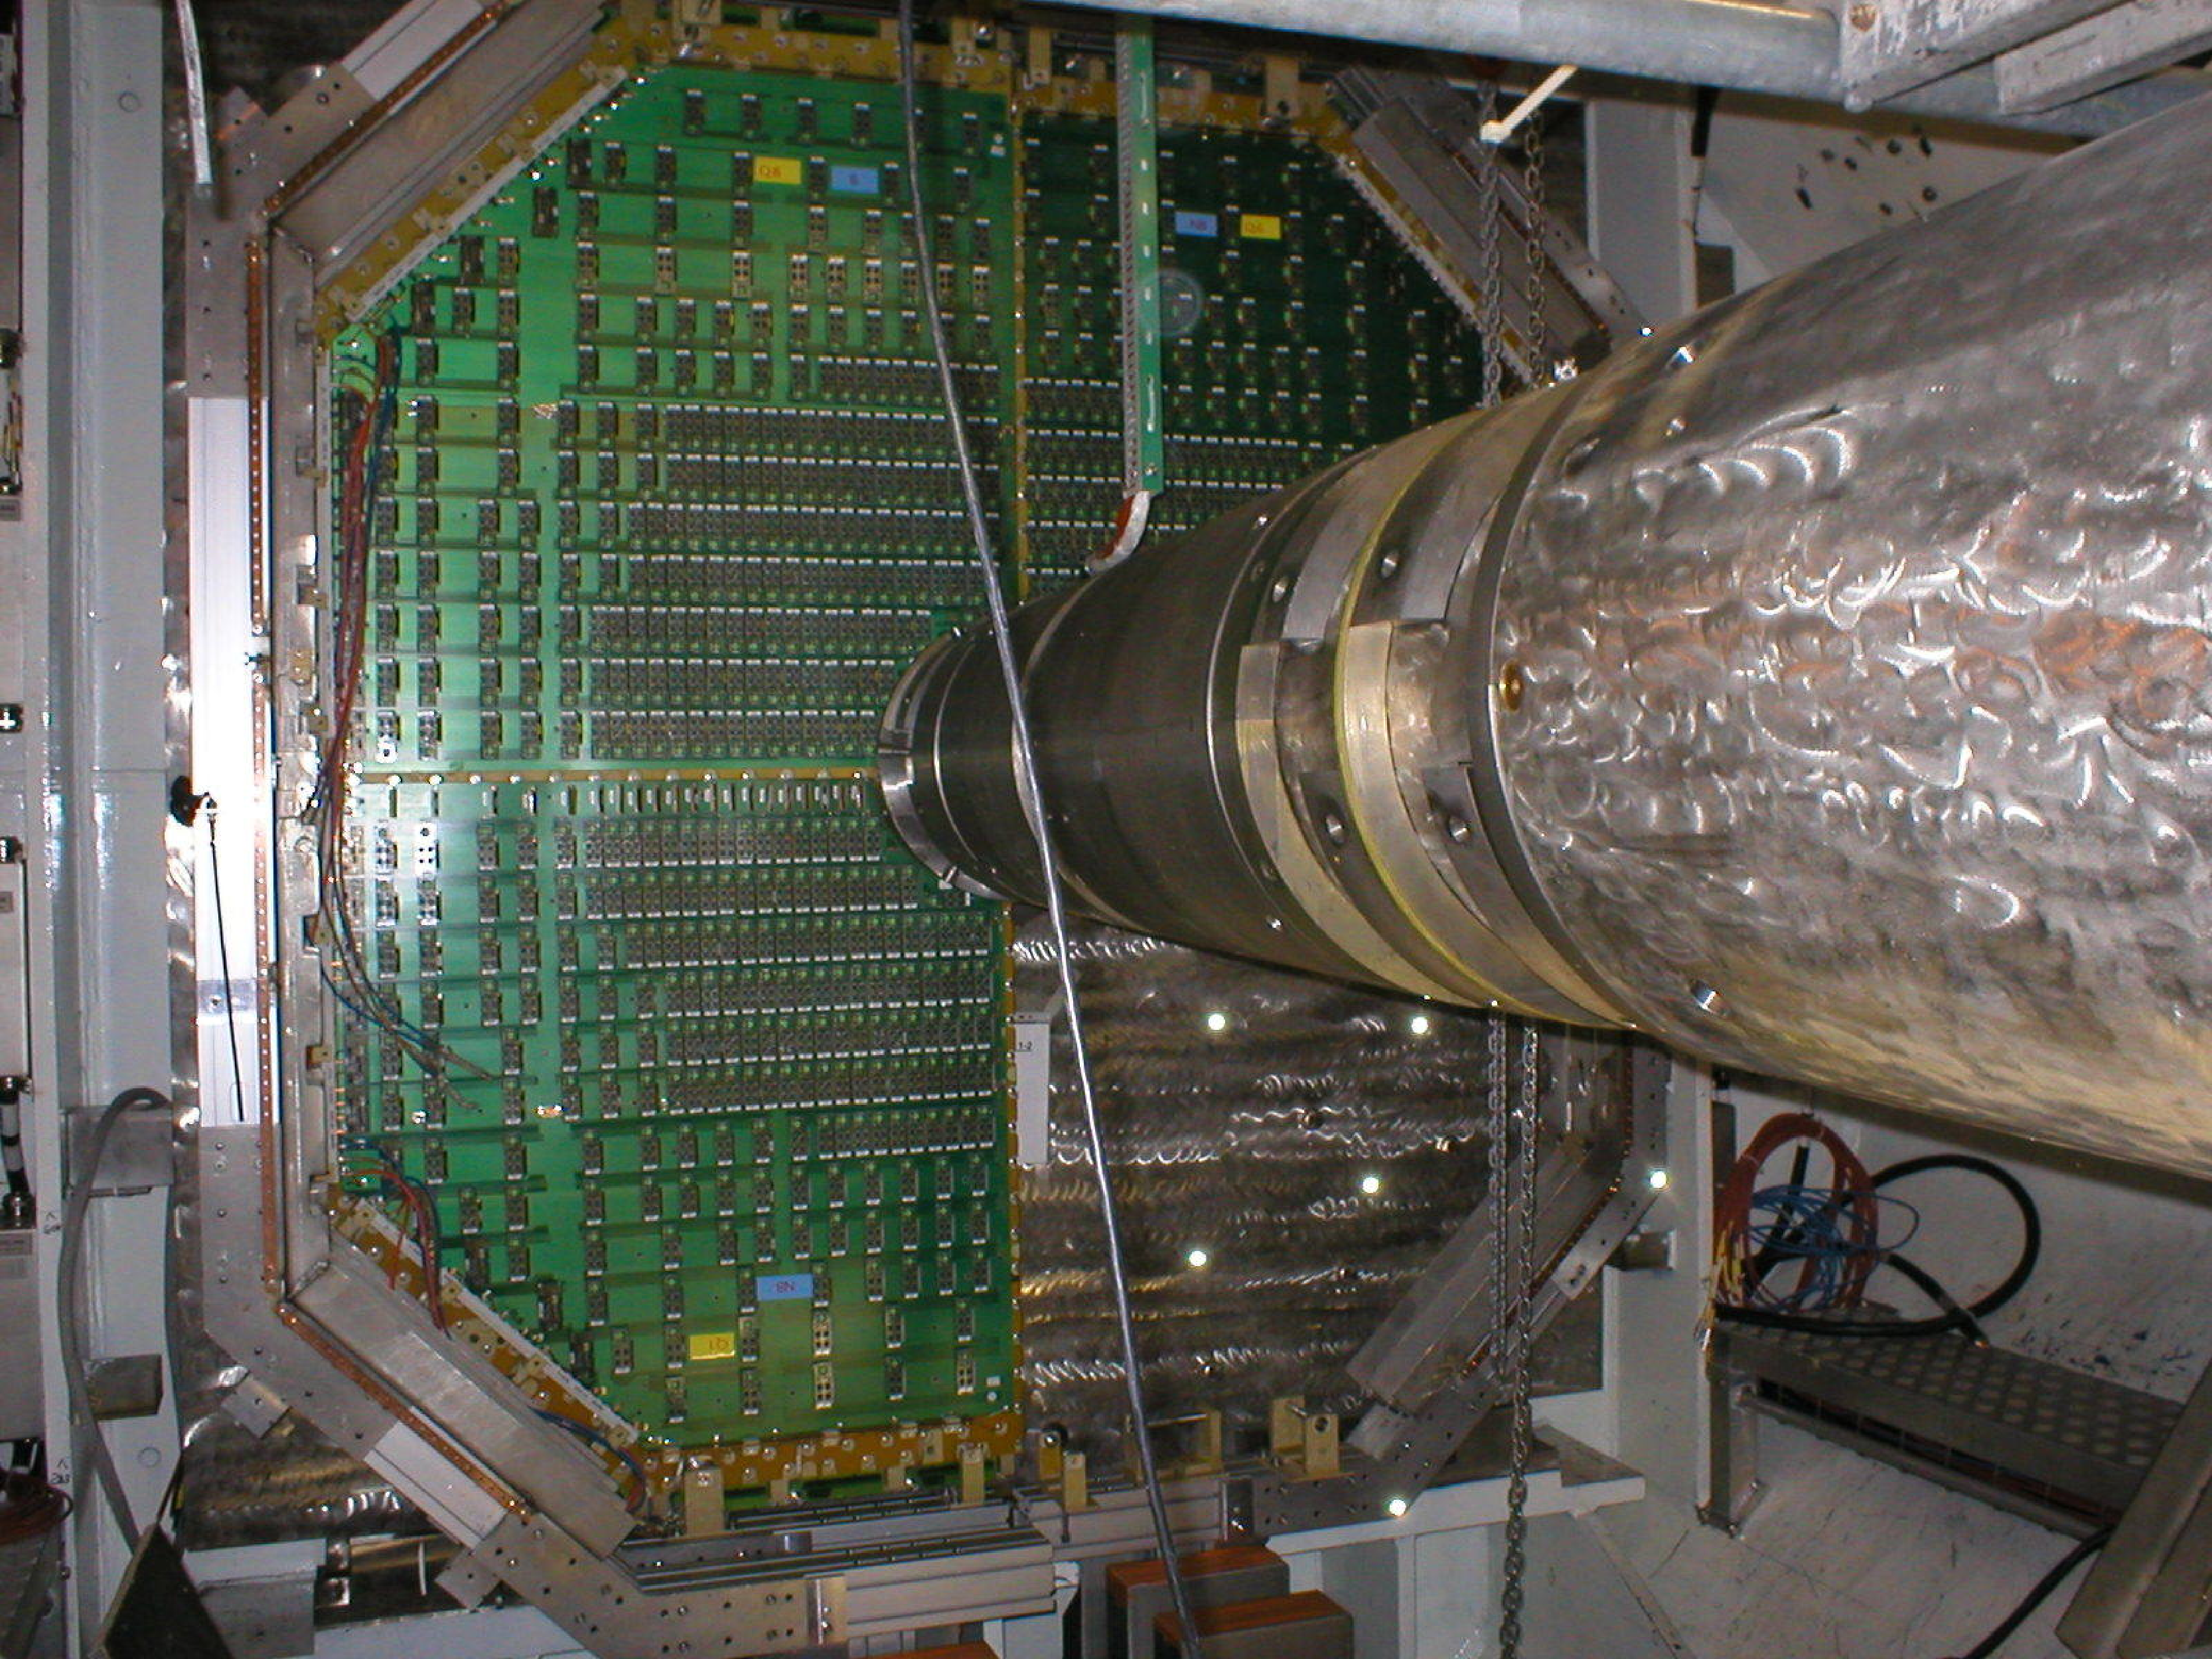
\includegraphics[scale=0.25]{images/MuonStation1.pdf}
} 
\end{frame}


\begin{frame}
\frametitle{Detector Structure Station1 quadrant}
\centering{
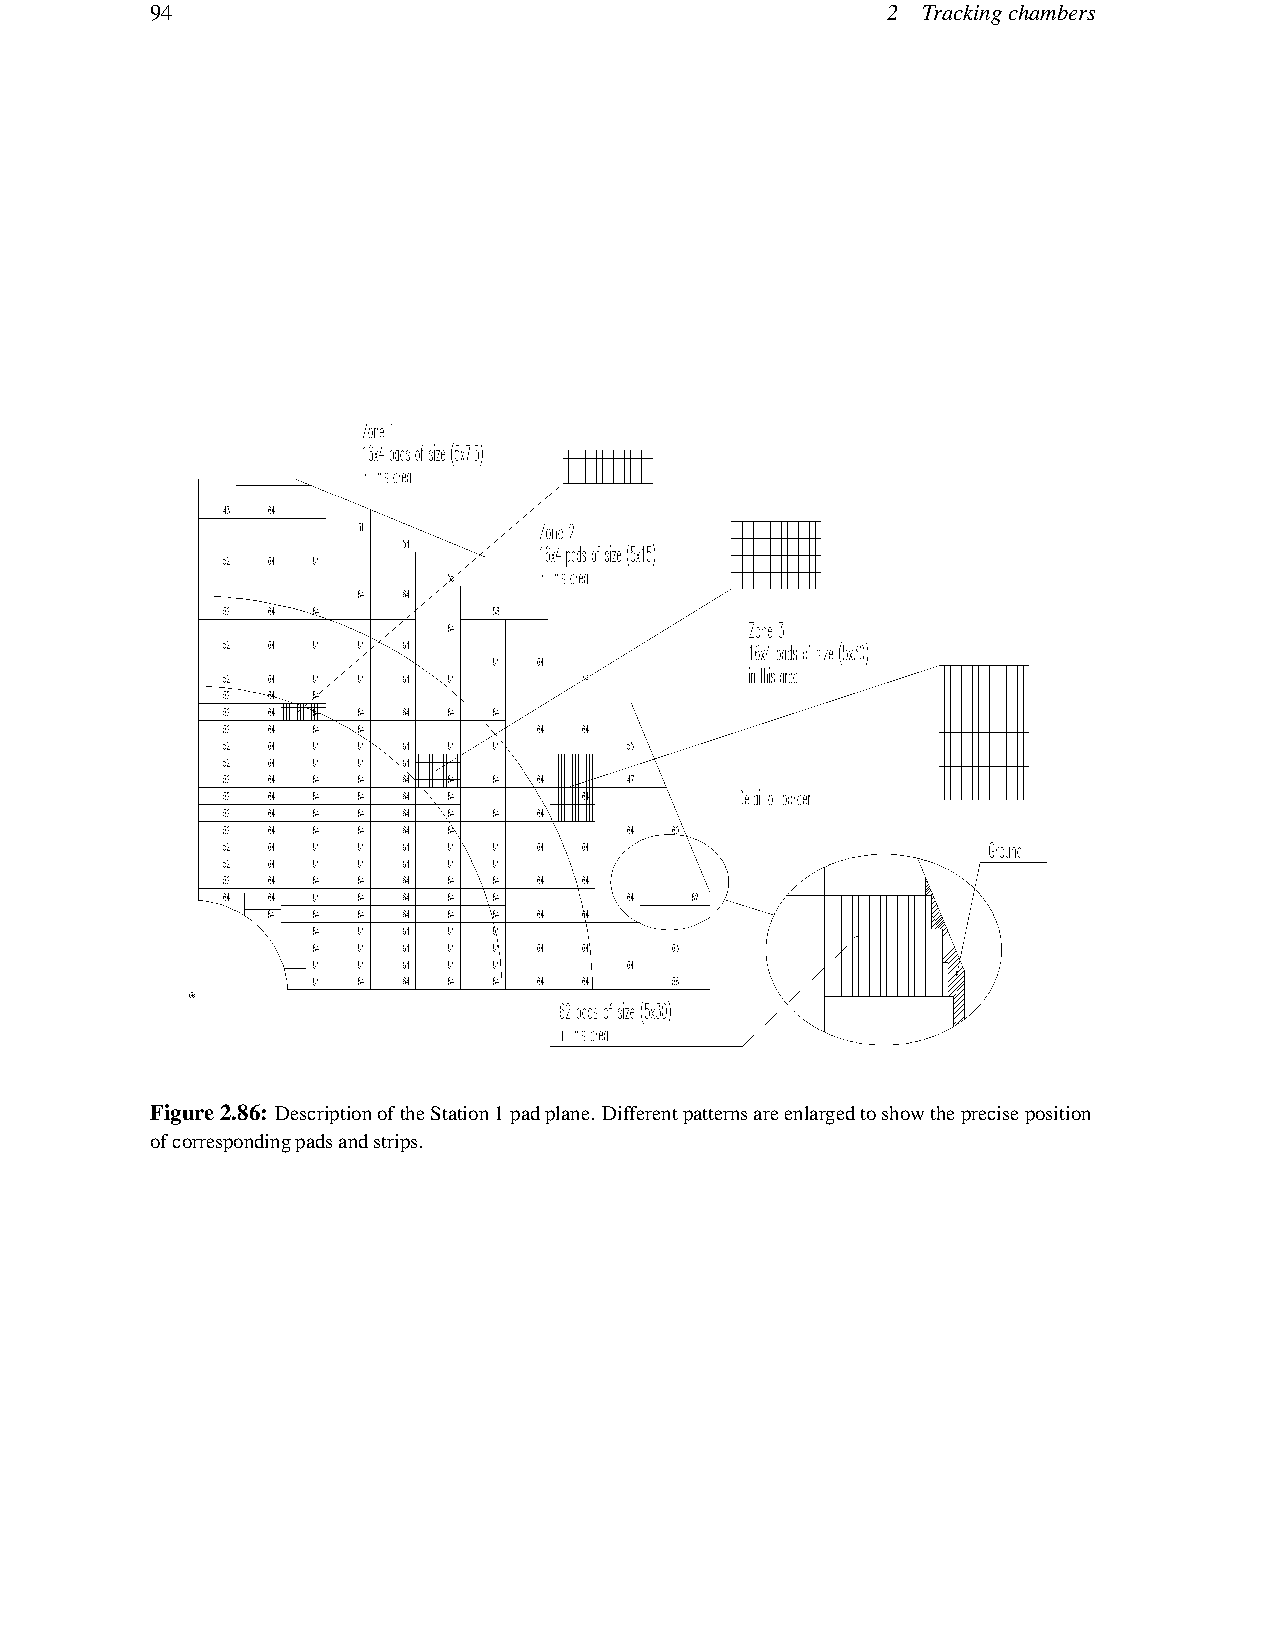
\includegraphics[scale=0.75,trim={2cm 7cm 3cm 7cm},clip]{images/Station1Wires.pdf}
} \\
\end{frame}

\begin{frame}
\frametitle{Detector Slats}
\centering{
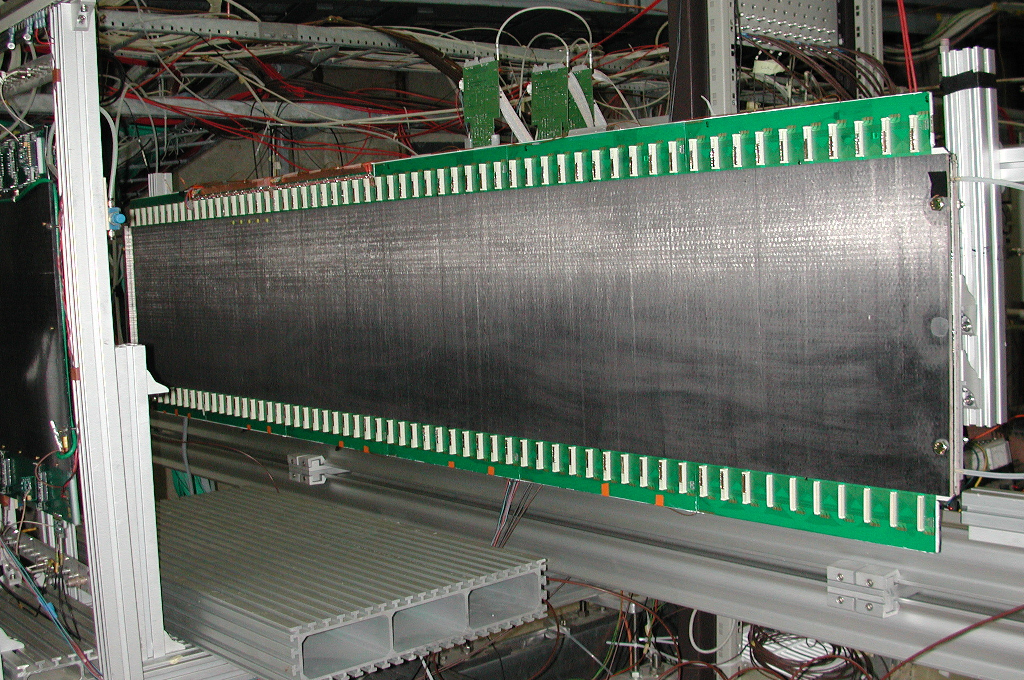
\includegraphics[scale=0.5]{images/MUONSlat.pdf}
} 
\end{frame}
%\begin{frame}
%\frametitle{Detector Slats in place}
%\centering{
%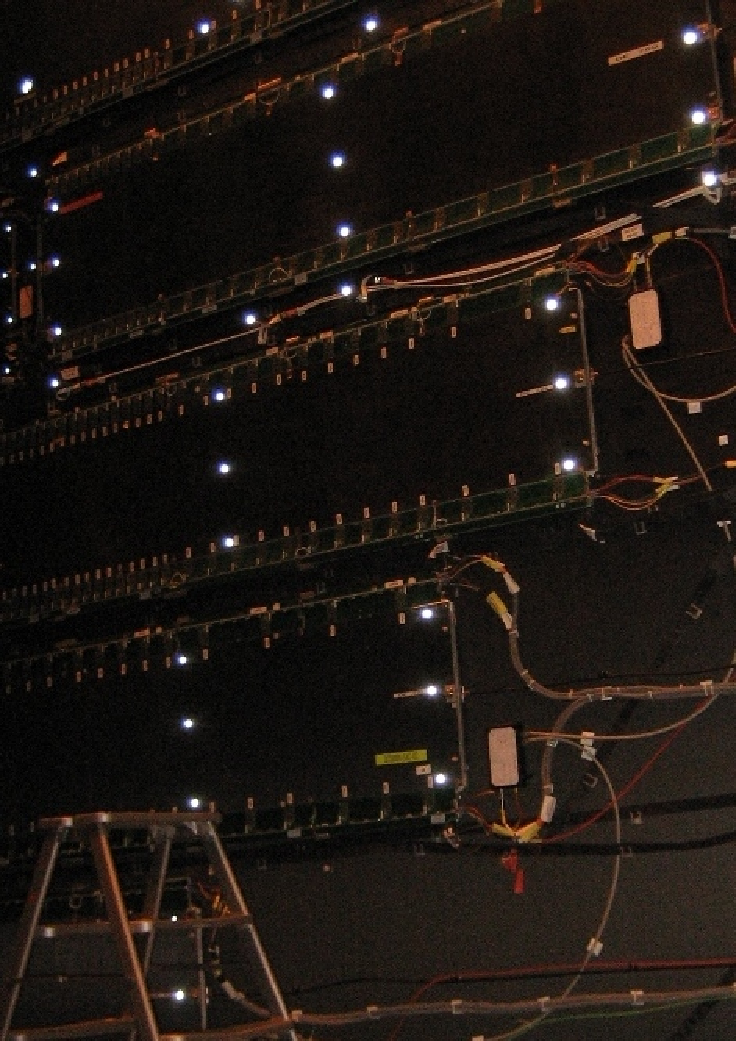
\includegraphics[scale=0.5]{images/MUONSlatsIn.pdf}
%} 
%\end{frame}


\begin{frame}
\frametitle{MUON Slats through the Dipole}
\centering{
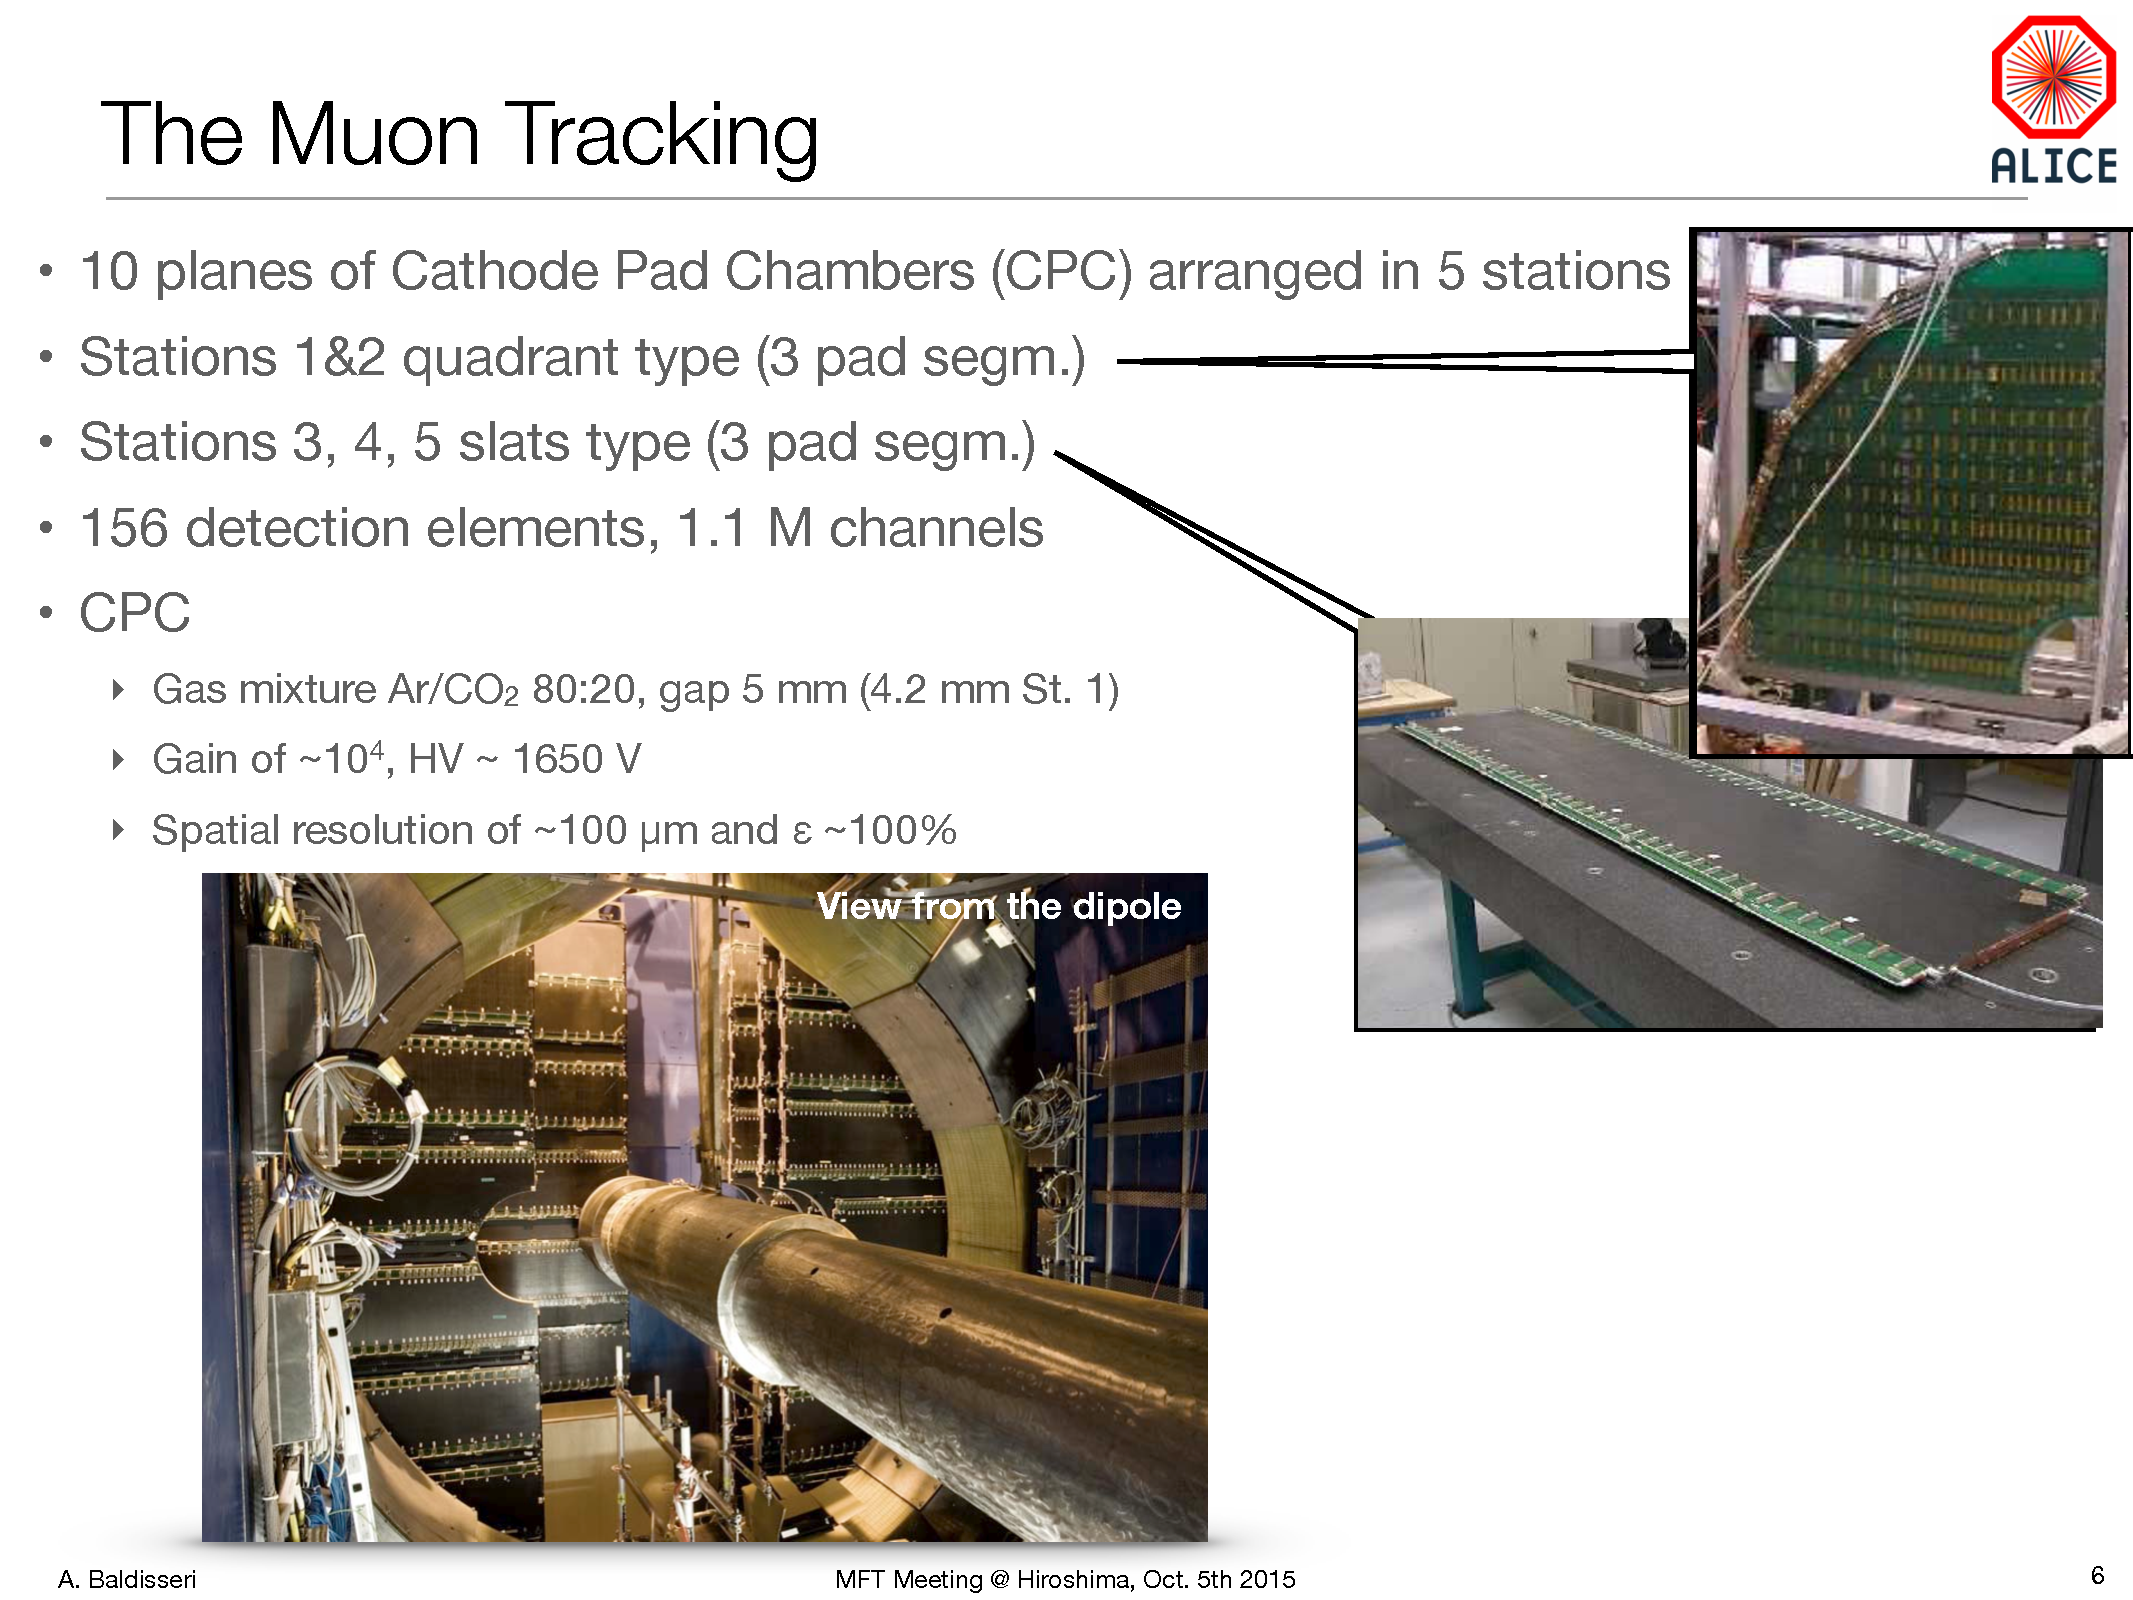
\includegraphics[scale=0.5, trim={2cm 1cm 17cm 16cm},clip]{images/pg_0006.pdf}
} \\

\end{frame}

\begin{frame}
\frametitle{Detector Slats schematic}
\centering{
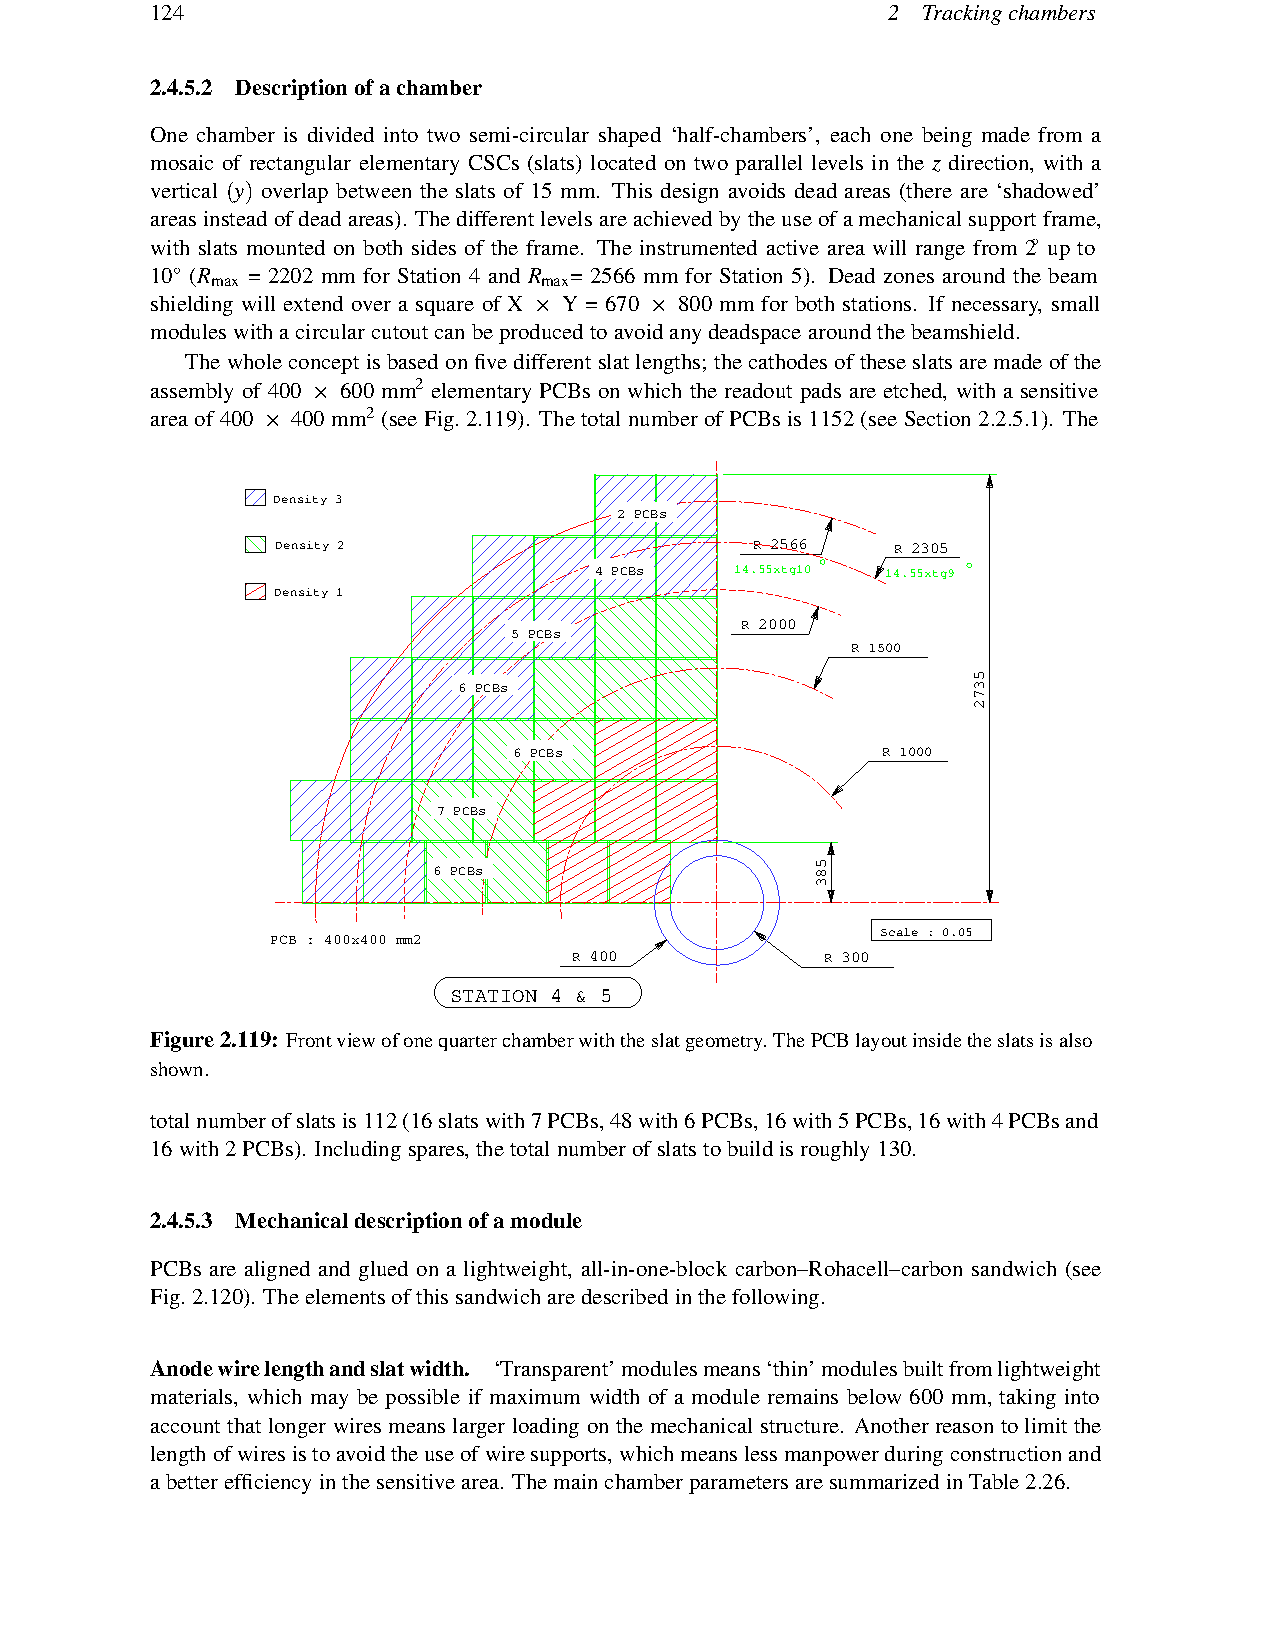
\includegraphics[scale=0.75, trim={4cm 10.5cm 2cm 8cm},clip]{images/Chapter2-2_pages_24.pdf}
} 
\end{frame}


\begin{frame}
  \frametitle{Nominal pp event}
\centering{
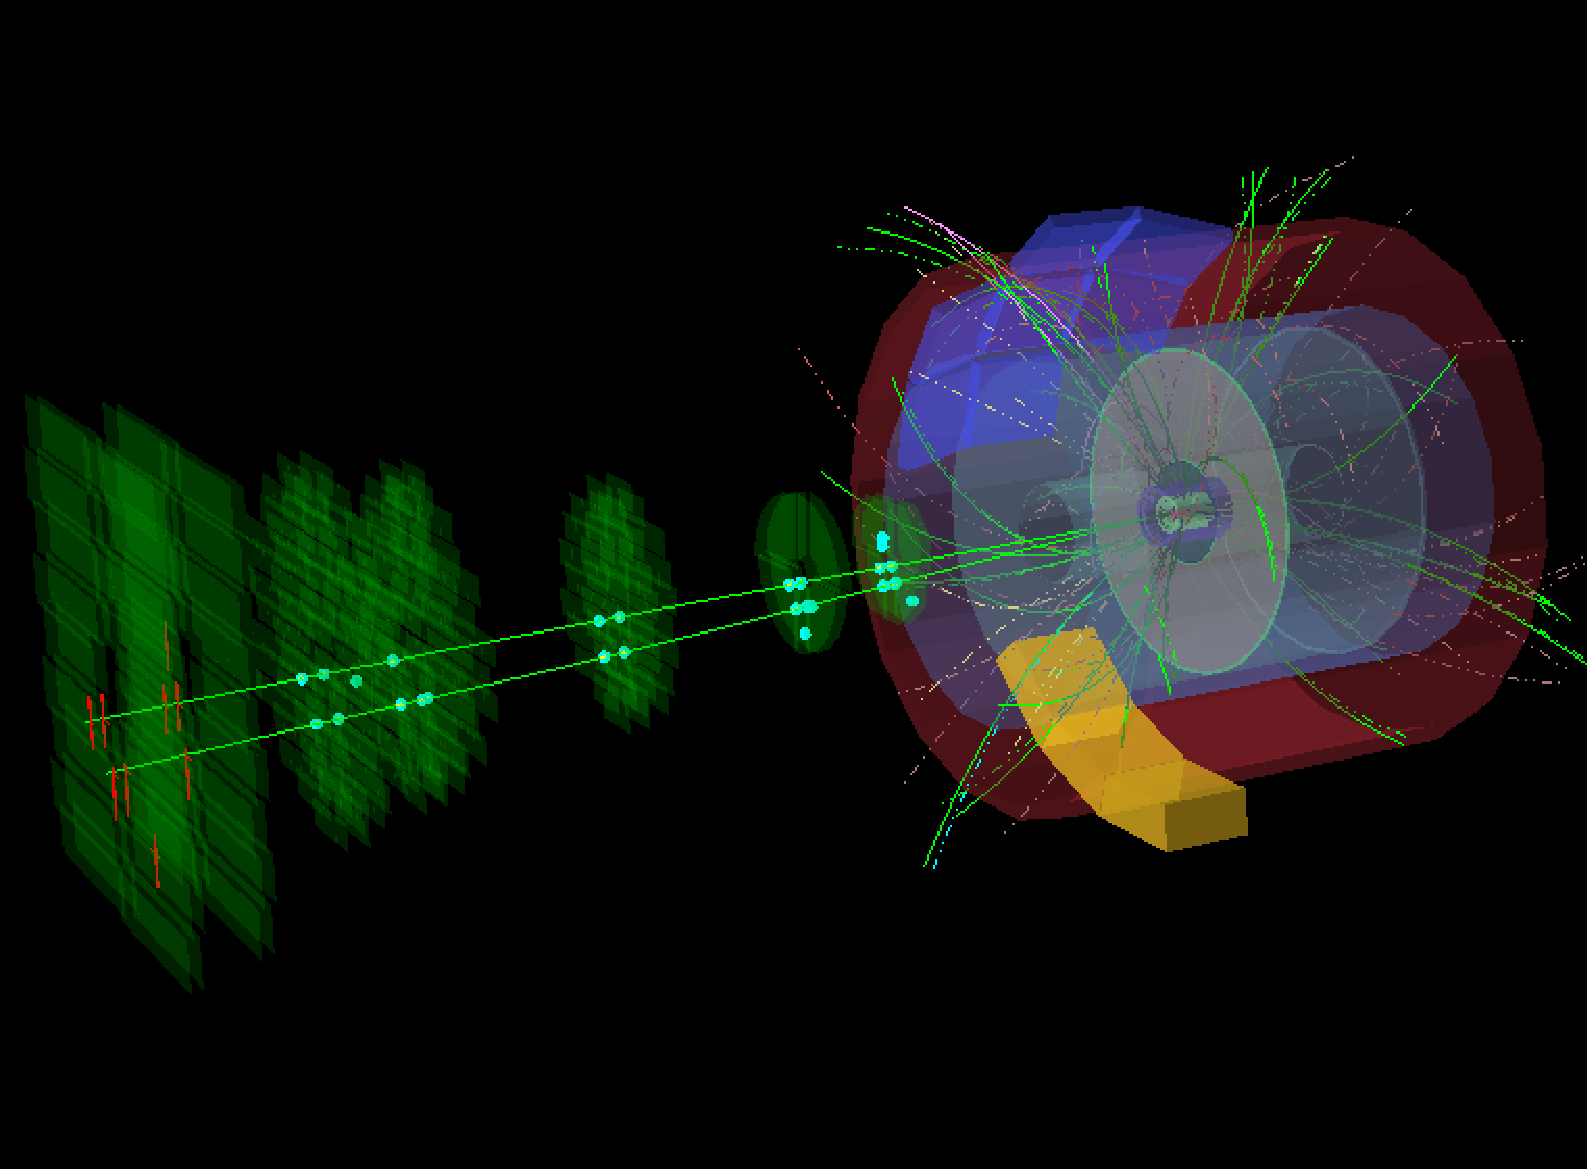
\includegraphics[scale=0.35]{images/7TeVALICEEvent.pdf}
} \\
pp at $\sqrt{s}$=7TeV, 2010 \\
Nucl.Phys. A862-863 (2011) 223-230
\end{frame}

\begin{frame}
  \frametitle{Nominal PbPb event}
\centering{
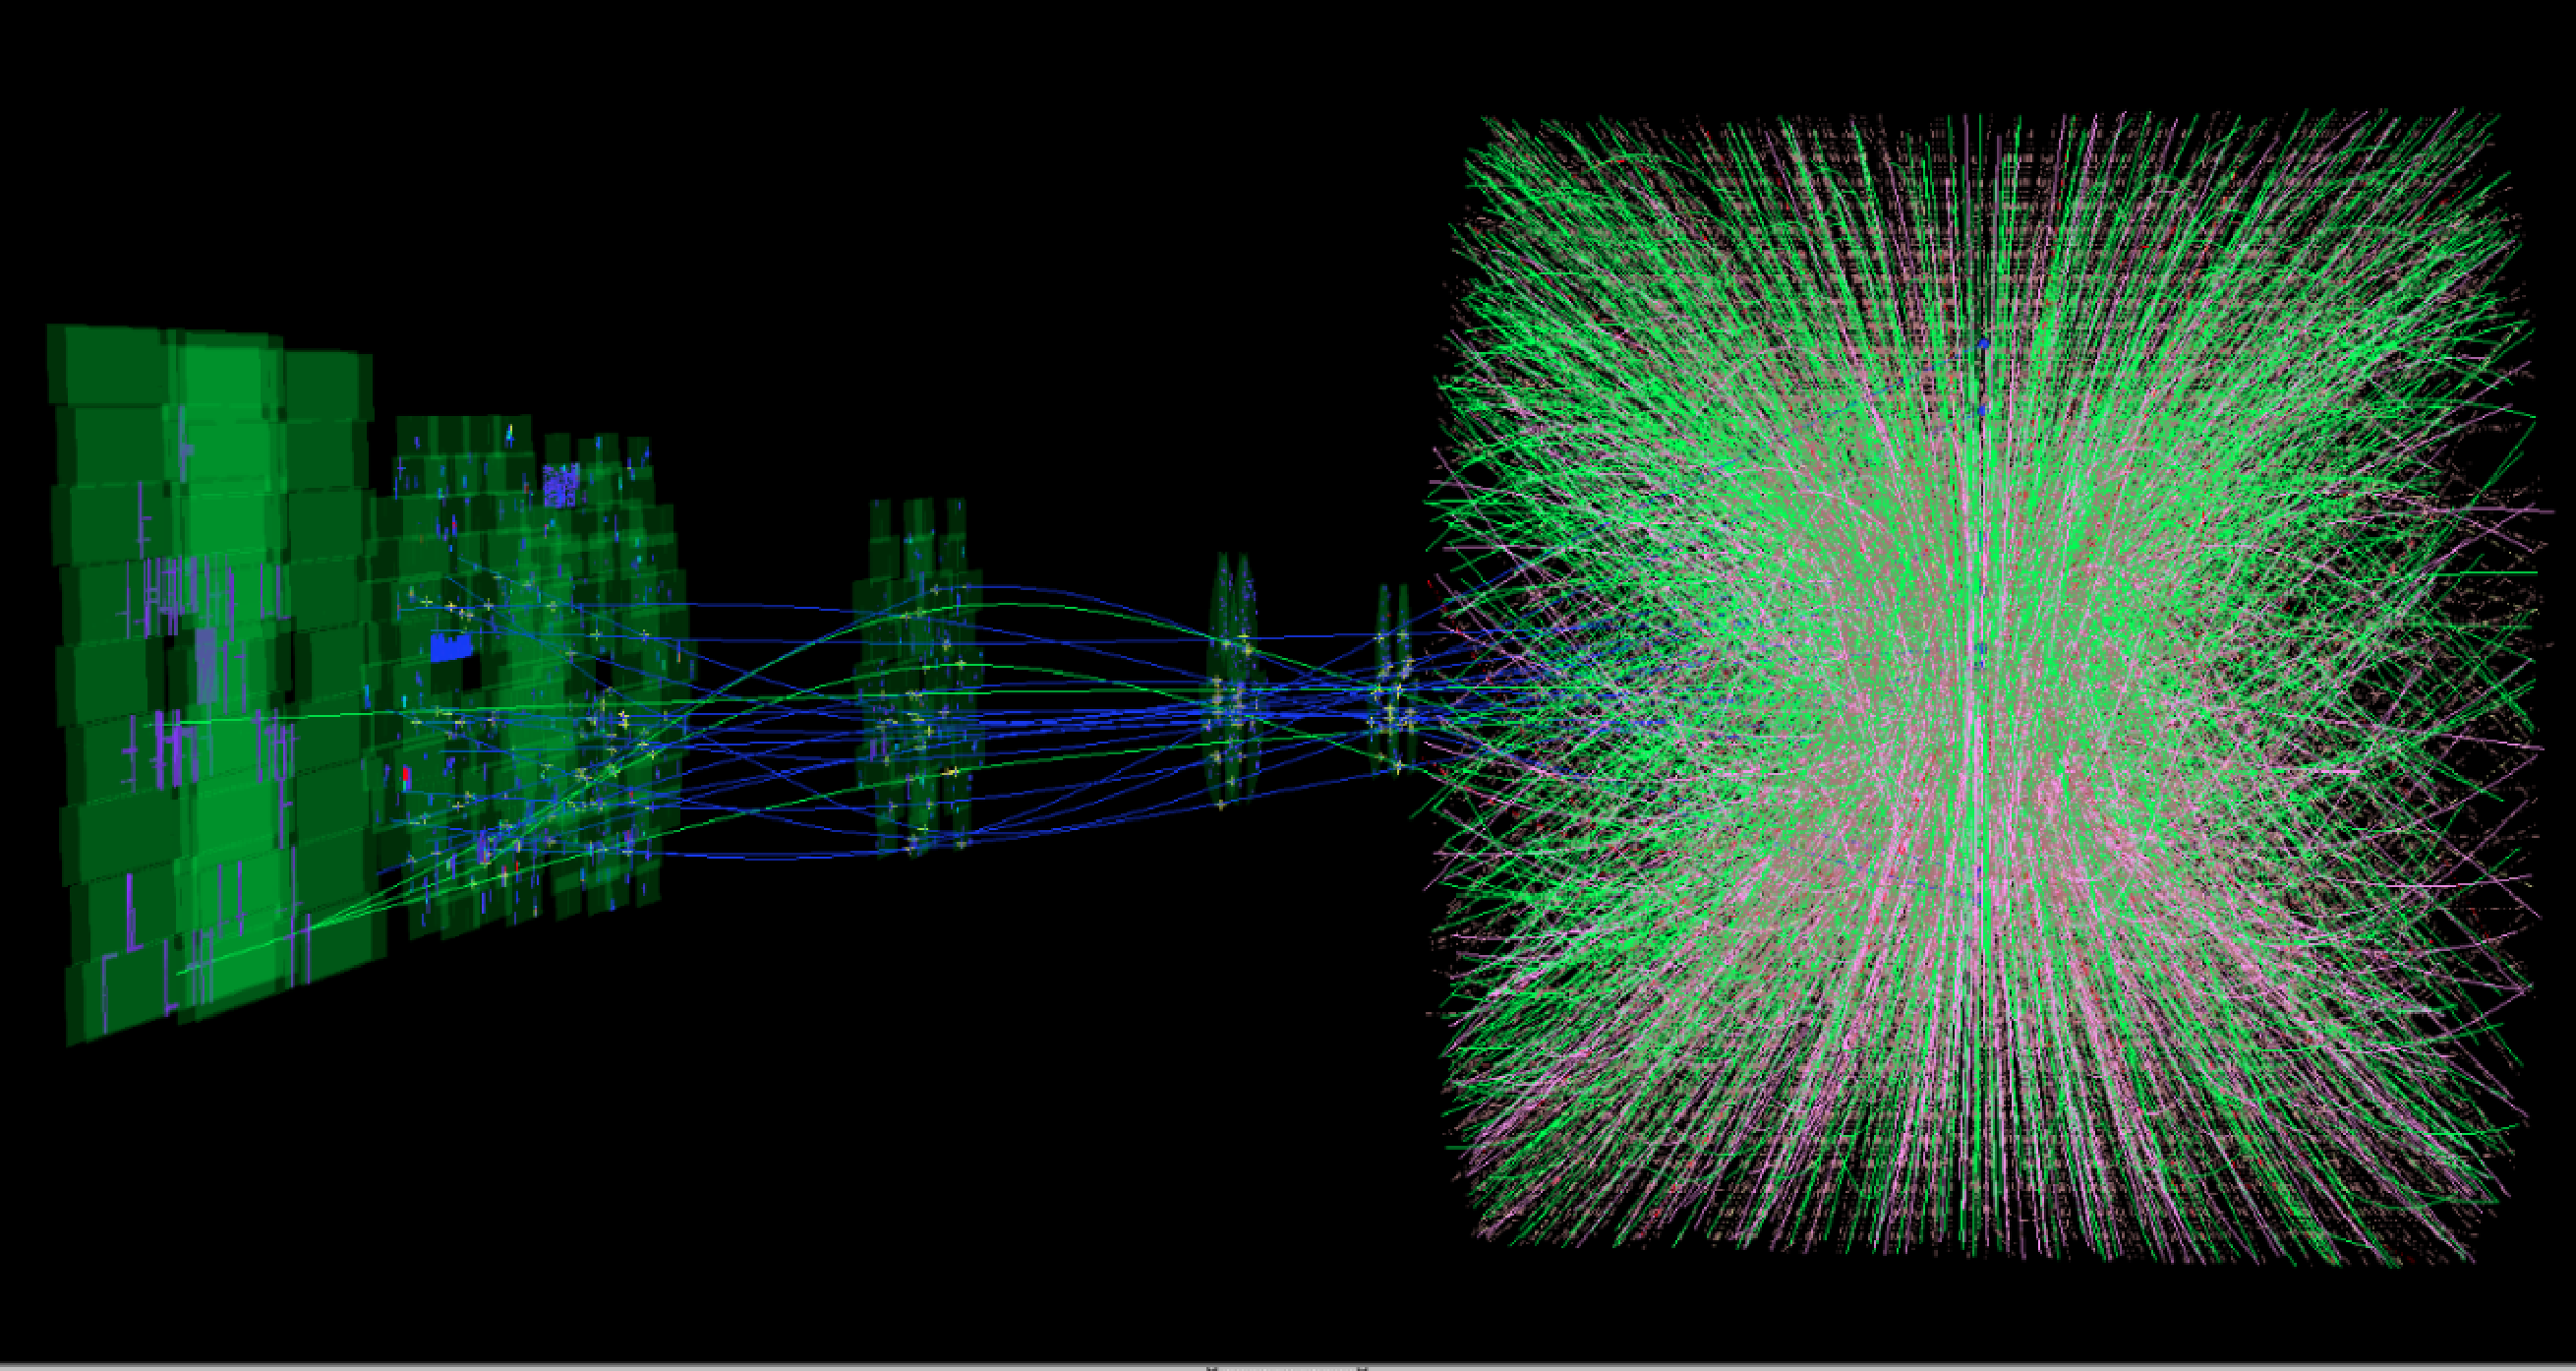
\includegraphics[scale=0.25]{images/HeavyIon.pdf}
} \\
PbPb at $\sqrt{s}$=7 TeV, 2015 \\
\end{frame}

\begin{frame}
  \frametitle{Diagram of detection}

\begin{columns}[T] % align columns
\begin{column}{.48\textwidth}
\begin{itemize}
  \item 100m$^2$ total area
  \item 1.4 million channels
  \item Wire diameter = 20$\mu m$
  \item Wire Pitch : 2$mm$ St1\\
    2.5$mm$ St 2,3,4,5
  \item Pad sizes \\
    \begin{enumerate}
      \item 5x7.5$mm$
      \item 5x15$mm$
      \item 5x30$mm$
    \end{enumerate}
\end{itemize}

\end{column}%
\hfill%
\begin{column}{.48\textwidth}
  \centering{
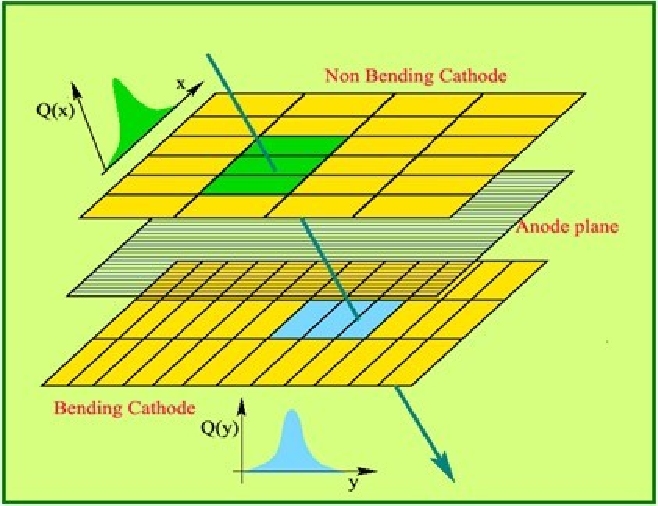
\includegraphics[scale=0.5, angle=90]{images/bendingnonbending.pdf}
} 

\end{column}%
\end{columns}  
  
  
  
\end{frame}


\section{Current MUON Software}

\begin{frame}
\frametitle{Current MUON reconstruction Software}
\begin{itemize}
  \item Raw Data Decoding
  \item Raw Data Filtering
  \item Pre Clustering 
  \item Clusterise, locate cluster interaction point.
  \item Tracking (MCH)
  \item Tracking (MID)
  \item Track Matching MCH-MID
\end{itemize}
\end{frame}

\begin{frame}
  \frametitle{where to start}
  \begin{quote}
\small{There is no doubt that the grail of efficiency leads to abuse. Programmers waste enormous amounts of time thinking about, or worrying about, the speed of noncritical parts of their programs, and these attempts at efficiency actually have a strong negative impact when debugging and maintenance are considered. We should forget about small efficiencies, say about 97\% of the time: premature optimization is the root of all evil.
Yet we should not pass up our opportunities in that critical 3\%. A good programmer will not be lulled into complacency by such reasoning, he will be wise to look carefully at the critical code; but only after that code has been identified.}  
  \end{quote}
Donald Knuth, ACM Computing Surveys, Vol 6, No. 4, Dec. 1974 (see p.268)
\end{frame}

\begin{frame}
  \frametitle{Time Spent}

\begin{tabular}{|l|r|r|r|}
  Function & \multicolumn{3}{c}{Time in \%} \\  
  & pp 16  & PbPb 11 & PbPb 15\\ \hline 
% uncover makes advanced overlay
Raw Data Decoding & 4 & &\\
Raw Data Filtering & 2 & &\\
Pre Clustring & 10 & &\\
Clustering & 63 & & \\
Tracking MCH & 7 & & \\
Tracking MID & 6 & & \\
Track matching & 8 & & \\
\end{tabular}\\
\vspace{2cm}
\end{frame}

\begin{frame}
  \frametitle{Graphically}
  include graphic of table.
\end{frame}
\section{Cluster Finder}

\begin{frame}
\frametitle{What is a cluster finder} 
picture of a couple of clusters.
\end{frame}

\begin{frame}
  \frametitle{MLEM Algorithm}
explain mlem
\end{frame}

\begin{frame}
  \frametitle{MLEM }

\end{frame}


\begin{frame}
  \frametitle{Logical Parts}
  \begin{itemize}
    \item Add Virtual pads if necessary  
    \item Find Center of Gravity given maximal pixel
    \item MLEM
  \end{itemize}
\end{frame}

\begin{frame}
  \frametitle{Effect of not adding Virtual Pads}
graph of radius of like clusters.
\end{frame}

\begin{frame}
  \frametitle{Effect of limiting the convergence to 5}
graph of radius of like clusters.
\end{frame}

\begin{frame}
  \frametitle{Speed up}
\begin{itemize}
  \item look for dead code
  \item change data or reorder to hit caches better.
  \item get a faster cpu. sadly not going to happen
  \item gpu x3 
  \item fpga - try to avoid.
\end{itemize}
Performed on a i7 with nvidia gtx 980, will have to be repeated on other hardware.
\end{frame}

\begin{frame}
\frametitle{Something else}
Look at the physics, and figure out a way to optimise based on the physics \ldots
\end{frame}

\end{document}

